\documentclass[UTF8]{ctexart}

% font packages
\usepackage{amsfonts}
\usepackage{amssymb}
\usepackage{amsthm}
\usepackage{amsmath}
\usepackage{mathrsfs}

% margin
\usepackage{geometry}
\geometry{
    paper =a4paper,
    top =3cm,
    bottom =3cm,
    left=2cm,
    right =2cm
}
\linespread{1.2}

% more math operators' support
\usepackage{physics}

% Boldface
\usepackage{bm}

% Tikz
\usepackage{tikz}
\usetikzlibrary{calc}

% Gaussian Elimination
\usepackage{gauss}

% Commutative Graph
\usepackage[all]{xy}

% Comment
\usepackage{comment}

% Colors
\usepackage{xcolor}

% 文字颜色的命令
\newcommand{\tc}[4][white]{{\fcolorbox{#1}{#2}{\textcolor{#3}{#4}}}} % 此命令接受四个参数,第一个参数为边框颜色,默认为白色,第二个参数为文字背景颜色,第三个参数为文字颜色,第四个参数为文字内容。如:\tc[green]{blue}{lime}{Hello,world!}

% Reference support
\usepackage{hyperref}
\hypersetup{
    colorlinks=true,
    linkcolor=blue,
    filecolor=magenta,
    urlcolor=cyan
} % 请在此处自定义链接的颜色,相当于\textcolor

% Info
\title{Title}
\author{Fulcrum4Math}
\date{\today}

% General
\DeclareMathOperator{\N}{\mathbb{N}}                    % Set of Natural Numbers
\DeclareMathOperator{\Z}{\mathbb{Z}}                    % Set of Integers
\DeclareMathOperator{\Q}{\mathbb{Q}}                    % Set of Rational Numbers
\DeclareMathOperator{\R}{\mathbb{R}}                    % Set of Real Numbers
\DeclareMathOperator{\C}{\mathbb{C}}                    % Set of Complex Numbers

\DeclareMathOperator{\Id}{Id}                           % Identity

\DeclareMathOperator{\Ker}{Ker}                         % Kernel of a Homomorphism ($\ker$ is included in package amsmath)
\DeclareMathOperator{\Image}{Im}                        % Image of a mapping

% Mathematical Logic
\DeclareMathOperator{\true}{\mathbb{T}}                    % Tautology
\DeclareMathOperator{\false}{\mathbb{F}}                    % Contradictory Formula
% Set Theory
\DeclareMathOperator{\PP}{\mathcal{P}}                  % Power Sets
\DeclareMathOperator{\card}{card}                       % Cardinality

% Category Theory
\DeclareMathOperator{\Cat}{\mathcal{C}}                 % Category

\DeclareMathOperator{\Hom}{Hom}                         % Set of Homomorphisms
\DeclareMathOperator{\End}{End}                         % Set of Endomorphisms
\DeclareMathOperator{\Aut}{Aut}                         % Set of Automorphisms
\DeclareMathOperator{\Isom}{Isom}                       % Set of Isomorphisms

\DeclareMathOperator{\Ob}{Ob}                           % Objects of a Category
\DeclareMathOperator{\Mor}{Mor}                         % Morphisms of a Category

% Abstract Algebra

\DeclareMathOperator{\stab}{stab}

% Topology
\DeclareMathOperator{\T}{\mathcal{T}}                   % Topology

\DeclareMathOperator{\intr}{int}                        % Interior
\DeclareMathOperator{\cl}{cl}                           % Closure

\DeclareMathOperator{\U}{\overset{\circ}{\mathit{U}}}   % Deleted Neighbourhood

% Linear Algebra

% \rank is included in package physics.
% \tr is included in package physics.

\DeclareMathOperator{\K}{\mathbb{K}}                    % Number Field
\DeclareMathOperator{\F}{\mathbb{F}}                    % Number Field (F)

\DeclareMathOperator{\diag}{\text{diag}}                % Diagonal Matrix
\DeclareMathOperator{\al}{\bm\alpha}                    % Boldfaced vector alpha
\DeclareMathOperator{\bt}{\bm\beta}                     % Boldfaced vector beta
\DeclareMathOperator{\x}{\bm{x}}                        % Boldfaced vector x
\DeclareMathOperator{\0}{\mathbf{0}}                    % Boldfaced vector x

\newcommand{\Jd}[2]{\mathrm{J}_{#1}{(#2)}}              % Jordan Blocks

% \DeclareMathOperator{\A}{\bm{A}}                    % Boldfaced matrix A
% \DeclareMathOperator{\B}{\bm{B}}                    % Boldfaced matrix B
% \DeclareMathOperator{\Cc}{\bm{C}}                   % Boldfaced matrix C

\DeclareMathOperator{\CCol}{Col}                        % Column Space
\DeclareMathOperator{\RRow}{Row}                        % Row Space
\DeclareMathOperator{\Null}{Null}                       % Null Space
\DeclareMathOperator{\rmT}{\mathrm{T}}                  % Transpose

\newcommand{\spn}{\mathrm{span}\text{ }}             % Span
% The original command `\span` leads to the environment `align` misdirected.

\DeclareMathOperator{\adj}{adj}                         % adj Matrix

\newcommand{\GL}[2]{\mathrm{GL}_{#1}(#2)}               % General Linear Group
\newcommand{\SL}[2]{\mathrm{SL}_{#1}(#2)}               % Special Linear Group

\DeclareMathOperator{\lcm}{lcm}                         % LCM

\newcommand{\<}{\langle}                                
\renewcommand{\>}{\rangle}                              % These two for ordinary Hilbert Inner Products <x,y>
\newcommand{\inprod}[2]{\<#1,#2\>}    % Using $\expval{#1}$ (Included in package physics) can replace \<#1\>.
\newcommand{\ocinterval}[2]{\left(#1,#2\right]}
\newcommand{\cointerval}[2]{\left[#1,#2\right)}
\newcommand{\ccinterval}[2]{\left[#1,#2\right]}
\newcommand{\oointerval}[2]{\left(#1,#2\right)}

% Mathematical Analysis

\DeclareMathOperator*{\ulim}{\overline{\lim}}
\DeclareMathOperator*{\llim}{\underline{\lim}}
\newcommand{\diff}[3]{\left. #1 \right|_{#2}^{#3}}    % This command can be replaced by $\eval{#1}_{#2}^{#3}$ in package physics.

\newcommand{\Ball}[2]{\mathcal{B}\left(#1,#2\right)}	% Open Ball

% Theorem template below copied from https://zhuanlan.zhihu.com/p/763738880

% ————————————————————————————————————自定义颜色————————————————————————————————————
\definecolor{dfn_green1}{RGB}{0, 156, 39} % 深绿
\definecolor{dfn_green2}{RGB}{214, 254, 224} % 浅绿

\definecolor{thm_blue1}{RGB}{0, 91, 156} % 深蓝
\definecolor{thm_blue2}{RGB}{218, 240, 255} % 浅蓝

\definecolor{ppt_pink1}{RGB}{172, 0, 175} % 深粉
\definecolor{ppt_pink2}{RGB}{255, 237, 255} % 浅粉

\definecolor{crl_orange1}{RGB}{225, 124, 0} % 深橙
\definecolor{crl_orange2}{RGB}{255, 235, 210} % 浅橙

\definecolor{xmp_purple1}{RGB}{119, 0, 229} % 深紫
\definecolor{xmp_purple2}{RGB}{239, 223, 255} % 浅紫

\definecolor{cxmp_red1}{RGB}{211, 0, 35} % 深红
\definecolor{cxmp_red2}{RGB}{255, 214, 220} % 浅红

\definecolor{prf_grey1}{RGB}{120, 120, 120} % 深灰
\definecolor{prf_grey2}{RGB}{233, 233, 233} % 浅灰

\definecolor{axm_yellow1}{RGB}{192, 192, 0} % 深黄
\definecolor{axm_yellow2}{RGB}{255, 255, 172} % 浅黄

% 将RGB换为rgb,颜色数值取值范围改为0到1
% ————————————————————————————————————自定义颜色————————————————————————————————————

% ————————————————————————————————————盒子设置————————————————————————————————————

\usepackage{tcolorbox} % 盒子效果
\tcbuselibrary{most} % tcolorbox宏包的设置,详见宏包说明文档

% tolorbox提供了tcolorbox环境,其格式如下:
% 第一种格式:\begin{tcolorbox}[colback=⟨背景色⟩, colframe=⟨框线色⟩, arc=⟨转角弧度半径⟩, boxrule=⟨框线粗⟩]   \end{tcolorbox}
% 其中设置arc=0mm可得到直角;boxrule可换为toprule/bottomrule/leftrule/rightrule可分别设置对应边宽度,但是设置为0mm时仍有细边,若要绘制单边框线推荐使用第二种格式
% 方括号内加上title=⟨标题⟩, titlerule=⟨标题背景线粗⟩, colbacktitle=⟨标题背景线色⟩可为盒子加上标题及其背景线
% 第二种格式:\begin{tcolorbox}[enhanced, colback=⟨背景色⟩, boxrule=0pt, frame hidden, borderline={⟨框线粗⟩}{⟨偏移量⟩}{⟨框线色⟩}]   {\end{tcolorbox}}
% 将borderline换为borderline east/borderline west/borderline north/borderline south可分别为四边添加框线,同一边可以添加多条
% 加入breakable属性可以支持盒子拆分到两页中。
% 偏移量为正值时,框线向盒子内部移动相应距离,负值反之

\newenvironment{dfn_box}{
    \begin{tcolorbox}[enhanced, colback=dfn_green2, boxrule=0pt, frame hidden,
        borderline west={0.7mm}{0.1mm}{dfn_green1},breakable]
    }
    {\end{tcolorbox}}
    
\newenvironment{thm_box}{
    \begin{tcolorbox}[enhanced, colback=thm_blue2, boxrule=0pt, frame hidden,
        borderline west={0.7mm}{0.1mm}{thm_blue1},breakable]
    }
    {\end{tcolorbox}}
    
\newenvironment{ppt_box}{
    \begin{tcolorbox}[enhanced, colback=ppt_pink2, boxrule=0pt, frame hidden,
        borderline west={0.7mm}{0.1mm}{ppt_pink1},breakable]
    }
    {\end{tcolorbox}}
    
\newenvironment{crl_box}{
    \begin{tcolorbox}[enhanced, colback=crl_orange2, boxrule=0pt, frame hidden,
        borderline west={0.7mm}{0.1mm}{crl_orange1},breakable]
    }
    {\end{tcolorbox}}
    
\newenvironment{xmp_box}{
    \begin{tcolorbox}[enhanced, colback=xmp_purple2, boxrule=0pt, frame hidden,
        borderline west={0.7mm}{0.1mm}{xmp_purple1},breakable]
    }
    {\end{tcolorbox}}
    
\newenvironment{cxmp_box}{
    \begin{tcolorbox}[enhanced, colback=cxmp_red2, boxrule=0pt, frame hidden,
        borderline west={0.7mm}{0.1mm}{cxmp_red1},breakable]
    }
    {\end{tcolorbox}}
    
\newenvironment{prf_box}{
    \begin{tcolorbox}[enhanced, colback=prf_grey2, boxrule=0pt, frame hidden,
        borderline west={0.7mm}{0.1mm}{prf_grey1},breakable]
    }
    {\end{tcolorbox}}
    
\newenvironment{axm_box}{
    \begin{tcolorbox}[enhanced, colback=axm_yellow2, boxrule=0pt, frame hidden,
        borderline west={0.7mm}{0.1mm}{axm_yellow1},breakable]
    }
    {\end{tcolorbox}}

% tcolorbox宏包还提供了\tcbox指令,用于生成行内盒子,可制作高光效果

        % \newcommand{\hl}[1]{
        %     \tcbox[on line, arc=0pt, colback=hlan!5!white, colframe=hlan!5!white, boxsep=1pt, left=1pt, right=1pt, top=1.5pt, bottom=1.5pt, boxrule=0pt]
        % {\bfseries \color{hlan}#1}}

% 其中on line将盒子放置在本行(缺失会跳到下一行),boxsep用于控制文本内容和边框的距离,left、right、top、bottom则分别在boxsep的参数的基础上分别控制四边距离

% ————————————————————————————————————盒子设置————————————————————————————————————

% ————————————————————————————————————定理类环境设置————————————————————————————————————
\newtheoremstyle{MyStyle}{0pt}{}{}{\parindent}{\bfseries}{}{1em}{} % 定义新定理风格。格式如下:
%\newtheoremstyle{⟨风格名⟩}
%                {⟨上方间距⟩} % 若留空,则使用默认值
%                {⟨下方间距⟩} % 若留空,则使用默认值
%                {⟨主体字体⟩} % 如 \itshape
%                {⟨缩进长度⟩} % 若留空,则无缩进;可以使用 \parindent 进行正常段落缩进
%                {⟨定理头字体⟩} % 如 \bfseries
%                {⟨定理头后的标点符号⟩} % 如点号、冒号
%                {⟨定理头后的间距⟩} % 不可留空,若设置为 { },则表示正常词间间距;若设置为 {\newline},则环境内容开启新行
%                {⟨定理头格式指定⟩} % 一般留空
% 定理风格决定着由 \newtheorem 定义的环境的具体格式,有三种定理风格是预定义的,它们分别是:
% plain: 环境内容使用意大利斜体,环境上下方添加额外间距
% definition: 环境内容使用罗马正体,环境上下方添加额外间距
% remark: 环境内容使用罗马正体,环境上下方不添加额外间距

\theoremstyle{MyStyle} % 设置定理风格 

% 定义定义环境,格式为\newtheorem{⟨环境名⟩}{⟨定理头文本⟩}[⟨上级计数器⟩]或\newtheorem{⟨环境名⟩}[⟨共享计数器⟩]{⟨定理头文本⟩},其变体\newtheorem*不带编号

% 以下的每个环境接受参数,请按顺序填入:
% #1 环境标题(中文)

\newtheorem{axiom}{公理}[section]
\newenvironment{axm}[2]
{
    \begin{axm_box}
        \begin{axiom}
            \textbf{#1
                \ifx\relax#2\relax\else % 检查 #2 是否为空
                    (#2) % 如果 #2 不为空,渲染 [空格](#2)
                \fi}
            \newline
}
{
        \end{axiom}
    \end{axm_box}
}

\newtheorem{definition}{定义}[subsection]
\newenvironment{dfn}[2]
{
    \begin{dfn_box}
        \begin{definition}
            \textbf{#1
                \ifx\relax#2\relax\else % 检查 #2 是否为空
                    (#2) % 如果 #2 不为空,渲染 [空格](#2)
                \fi}
            \newline
}
{
        \end{definition}
    \end{dfn_box}
}

\newtheorem{concept}[definition]{概念}
\newenvironment{cpt}[1]
{
    \begin{dfn_box}
        \begin{concept}
            \textbf{#1}
            \newline
}
{
        \end{concept}
    \end{dfn_box}
}

\newtheorem{syntax}[definition]{语法}
\newenvironment{syn}[1]
{
    \begin{thm_box}
        \begin{syntax}
            \textbf{#1}
            \newline
}
{
        \end{syntax}
    \end{thm_box}
}

\newtheorem{theorem}[definition]{定理}
\newenvironment{thm}[2]
{
    \begin{thm_box}
        \begin{theorem}
            \textbf{#1
                \ifx\relax#2\relax\else % 检查 #2 是否为空
                    (#2) % 如果 #2 不为空,渲染 [空格](#2)
                \fi}
            \newline
}
{
        \end{theorem}
    \end{thm_box}
}

\newtheorem{mytactic}{策略}
\newenvironment{tactic}[1]
{
    \begin{thm_box}
        \begin{mytactic}
            \textbf{#1}
            \newline
}
{
        \end{mytactic}
    \end{thm_box}
}

\newtheorem{myvariation}{Tactic 变体}[definition]
\newenvironment{tacticvar}[1]
{
    \begin{ppt_box}
        \begin{myvariation}
            \textbf{#1}
            \newline
}
{
        \end{myvariation}
    \end{ppt_box}
}

\newtheorem{example}{ 例\, }[subsection]
\newenvironment{xmp}[1]
{
    \begin{xmp_box}
        \begin{example}
            \textbf{#1}
            \newline
}
{
        \end{example}
    \end{xmp_box}
}

\newtheorem{cexample}{反例}[subsection]
\newenvironment{cxmp}[1]
{
    \begin{cxmp_box}
        \begin{cexample}
            \textbf{#1}
            \newline
}
{
        \end{cexample}
    \end{cxmp_box}
}

\newtheorem*{myproof}{证明: \newline}
\newenvironment{prf}{\begin{prf_box}\begin{myproof}}{\end{myproof}\end{prf_box}}

\newenvironment{crs}[4]
{
    \begin{thm_box}
        \textbf{课程 #1: #2}
        
        \ifx\relax#3\relax\else % 检查 #3 是否为空
            \textbf{主讲: }#3 % 如果 #3 不为空,渲染 [空格](#3)
        \fi
        
        \ifx\relax#4\relax\else % 检查 #4 是否为空
            \textbf{课程材料: }#4 % 如果 #4 不为空,渲染 [空格](#4)
        \fi

        \textbf{主要内容: }
}
{
    \end{thm_box}
}

\newtheorem{project}{课题}
\newenvironment{prj}[1]
{
    \begin{xmp_box}
        \begin{project}
            \textbf{#1}
            \newline
}
{
        \end{project}
    \end{xmp_box}
}

\usepackage{listings}
\newcommand{\smallsec}[1]{\paragraph{#1.}}
\lstset{
    basicstyle = \ttfamily,
}

% Define Colors: 
\definecolor{leanblue}{RGB}{0,0,255}
\colorlet{keyword}{leanblue}
\colorlet{punct}{leanblue}

\definecolor{sorry}{RGB}{255,0,0}
\definecolor{comment}{RGB}{0,128,0}
\definecolor{string}{RGB}{163,21,21}
\definecolor{num}{RGB}{9,134,88}

\definecolor{thname}{RGB}{121,94,38}

\definecolor{background}{HTML}{EEEEEE}
\definecolor{delim}{RGB}{20,105,176}

\newcommand*{\lean}[1]{\texttt{\color{blue}#1}}

\lstdefinelanguage{lean}{
    % Define Keywords: 
    alsoletter = {\#,\?,.},
    keywords = {
        import, 
        namespace, 
        end, 
        open, 
        variable, 
        Prop, 
        Type, 
        % Declarations: 
        protected, 
        class, 
        instance, 
        def, 
        axiom, 
        example, 
        theorem, 
        lemma, 
        fun, 
        by, 
        % Basics: 
        \#check, 
        \#leansearch, 
        \#eval, 
        % Tactics: 
        exact, 
            % FOL: 
            intro,
            intros, 
            rintro, 
            apply,
            refine, 
            apply?, 
            constructor, 
            rcases, 
            obtain, 
            use, 
            left, 
            right, 
            cases, 
            case, 
            by\_cases, 
            by\_contra, 
            contrapose, 
            contrapose!,
            % Others: 
            symm, 
            calc, 
            unfold, 
            have, 
            let, 
            rw, 
            at, 
            change, 
            show, 
        }, 
    keywords = [2]{sorry}, 
    %
    numbers=left,
    numberstyle=\color{num},
    %
    % morecomment = [l]{--},
    moredelim=[l][\color{comment}]{--}, % morecomment -> moredelim, so that Unicode characters can be used in comments. 
    moredelim=[is][\color{thname}]{\#tm\{}{\}}, 
    morecomment = [s]{/-}{-/},
    commentstyle = \color{comment}, 
    %
    stringstyle = \color{string}, 
    %
    stepnumber=1,
    numbersep=8pt,
    showstringspaces=false,
    breaklines=true,
    frame=lines,
    backgroundcolor=\color{background},
    literate=
    % Keywords
        {th\_name}{{{\color{thname}th\_name}}}{7}
    % Math Symbols
        {ℕ}{{\ensuremath{\mathbb{N}}}}{1}
        {ℤ}{{\ensuremath{\mathbb{Z}}}}{1}
        {ℝ}{{\ensuremath{\mathbb{R}}}}{1}
        {ℚ}{{\ensuremath{\mathbb{Q}}}}{1}
        {ℂ}{{\ensuremath{\mathbb{C}}}}{1}
        {∩}{{\ensuremath{\cap}}}{1}
        {∪}{{\ensuremath{\cup}}}{1}
        {⊂}{{\ensuremath{\subseteq}}}{1}
        {⊆}{{\ensuremath{\subseteq}}}{1}
        {⊄}{{\ensuremath{\nsubseteq}}}{1}
        {⊈}{{\ensuremath{\nsubseteq}}}{1}
        {⊃}{{\ensuremath{\supseteq}}}{1}
        {⊇}{{\ensuremath{\supseteq}}}{1}
        {⊅}{{\ensuremath{\nsupseteq}}}{1}
        {⊉}{{\ensuremath{\nsupseteq}}}{1}
        {∈}{{\ensuremath{\in}}}{1}
        {∉}{{\ensuremath{\notin}}}{1}
        {∋}{{\ensuremath{\ni}}}{1}
        {∌}{{\ensuremath{\notni}}}{1}
        {∅}{{\ensuremath{\emptyset}}}{1}
        {∫}{{\ensuremath{\int}}}{1}
        {∑}{{\ensuremath{\mathrm{\Sigma}}}}{1}
        {Π}{{\ensuremath{\mathrm{\Pi}}}}{1}
        {≤}{{\ensuremath{\leq}}}{1}
        {≥}{{\ensuremath{\geq}}}{1}
        {≠}{{\ensuremath{\neq}}}{1}
        {≈}{{\ensuremath{\approx}}}{1}
        {≡}{{\ensuremath{\equiv}}}{1}
        {≃}{{\ensuremath{\simeq}}}{1}
    % Greek Letters lowercase
        {α}{{\ensuremath{\mathrm{\alpha}}}}{1}
        {β}{{\ensuremath{\mathrm{\beta}}}}{1}
        {γ}{{\ensuremath{\mathrm{\gamma}}}}{1}
        {δ}{{\ensuremath{\mathrm{\delta}}}}{1}
        {ε}{{\ensuremath{\mathrm{\varepsilon}}}}{1}
        {ζ}{{\ensuremath{\mathrm{\zeta}}}}{1}
        {η}{{\ensuremath{\mathrm{\eta}}}}{1}
        {θ}{{\ensuremath{\mathrm{\theta}}}}{1}
        {ι}{{\ensuremath{\mathrm{\iota}}}}{1}
        {κ}{{\ensuremath{\mathrm{\kappa}}}}{1}
        {μ}{{\ensuremath{\mathrm{\mu}}}}{1}
        {ν}{{\ensuremath{\mathrm{\nu}}}}{1}
        {ξ}{{\ensuremath{\mathrm{\xi}}}}{1}
        {π}{{\ensuremath{\mathrm{\mathnormal{\pi}}}}}{1}
        {ρ}{{\ensuremath{\mathrm{\rho}}}}{1}
        {σ}{{\ensuremath{\mathrm{\sigma}}}}{1}
        {τ}{{\ensuremath{\mathrm{\tau}}}}{1}
        {φ}{{\ensuremath{\mathrm{\varphi}}}}{1}
        {χ}{{\ensuremath{\mathrm{\chi}}}}{1}
        {ψ}{{\ensuremath{\mathrm{\psi}}}}{1}
        {ω}{{\ensuremath{\mathrm{\omega}}}}{1}
    % Greek Letters UPPERCASE
        {Γ}{{\ensuremath{\mathrm{\Gamma}}}}{1}
        {Δ}{{\ensuremath{\mathrm{\Delta}}}}{1}
        {Θ}{{\ensuremath{\mathrm{\Theta}}}}{1}
        {Λ}{{\ensuremath{\mathrm{\Lambda}}}}{1}
        {Σ}{{\ensuremath{\mathrm{\Sigma}}}}{1}
        {Φ}{{\ensuremath{\mathrm{\Phi}}}}{1}
        {Ξ}{{\ensuremath{\mathrm{\Xi}}}}{1}
        {Ψ}{{\ensuremath{\mathrm{\Psi}}}}{1}
        {Ω}{{\ensuremath{\mathrm{\Omega}}}}{1}
    % Arrows
        {↦}{{\ensuremath{\mapsto}}}{1}
        {←}{{\ensuremath{\leftarrow}}}{1}
        {<-}{{\ensuremath{\leftarrow}}}{1}
        {→}{{\ensuremath{\rightarrow}}}{1}
        {->}{{\ensuremath{\rightarrow}}}{1}
        {↔}{{\ensuremath{\leftrightarrow}}}{1}
        {<->}{{\ensuremath{\leftrightarrow}}}{1}
        {⇒}{{\ensuremath{\Rightarrow}}}{1}
        {⟹}{{\ensuremath{\Longrightarrow}}}{1}
        {⇐}{{\ensuremath{\Leftarrow}}}{1}
        {⟸}{{\ensuremath{\Longleftarrow}}}{1}
        {Σ}{{\ensuremath{\Sigma}}}{1}
        {Π}{{\ensuremath{\Pi}}}{1}
        {∀}{{\ensuremath{\forall}}}{1}
        {∃}{{\ensuremath{\exists}}}{1}
        {λ}{{\ensuremath{\mathrm{\lambda}}}}{1}
        {∧}{{\ensuremath{\wedge}}}{1}
        {∨}{{\ensuremath{\vee}}}{1}
        {¬}{{\ensuremath{\neg}}}{1}
        {⊢}{{\ensuremath{\vdash}}}{1}
        {‖}{{\ensuremath{\|}}}{1}
    % subscripts
        {₁}{{\ensuremath{_1}}}{1}
        {₂}{{\ensuremath{_2}}}{1}
        {₃}{{\ensuremath{_3}}}{1}
        {₄}{{\ensuremath{_4}}}{1}
        {₅}{{\ensuremath{_5}}}{1}
        {₆}{{\ensuremath{_6}}}{1}
        {₇}{{\ensuremath{_7}}}{1}
        {₈}{{\ensuremath{_8}}}{1}
        {₉}{{\ensuremath{_9}}}{1}
        {₀}{{\ensuremath{_0}}}{1}
        {ᵢ}{{\ensuremath{_i}}}{1}
        {ⱼ}{{\ensuremath{_j}}}{1}
        {ₐ}{{\ensuremath{_a}}}{1}
        {⁻¹}{{\ensuremath{^{-1}}}}{1}
        {¹}{{\ensuremath{^1}}}{1}
        {ₙ}{{\ensuremath{_n}}}{1}
        {ₘ}{{\ensuremath{_m}}}{1}
        {ₚ}{{\ensuremath{_p}}}{1}
    % Others
        {↑}{{\ensuremath{\uparrow}}}{1}
        {↓}{{\ensuremath{\downarrow}}}{1}
        {⊢}{{\ensuremath{\vdash}}}{1}
        {|-}{{\ensuremath{\vdash}}}{1}
        {⊥}{{\ensuremath{\perp}}}{1}
        {∞}{{\ensuremath{\infty}}}{1}
        {∂}{{\ensuremath{\partial}}}{1}
        {√}{{\ensuremath{\sqrt}}}{1}
        {∘}{{\ensuremath{\circ}}}{1}
        {×}{{\ensuremath{\times}}}{1}
        {∆}{{\ensuremath{\triangle}}}{1}
        {⟨}{{\ensuremath{\color{leanblue}\langle}}}{1}
        {⟩}{{\ensuremath{\color{leanblue}\rangle}}}{1}
        {⦃}{{\ensuremath{\color{leanblue}\{\![}}}{1}
        {⦄}{{\ensuremath{\color{leanblue}]\!\}}}}{1}
        {ℒ}{{\ensuremath{\mathscr{L}}}}{1}
        {𝒫}{{\ensuremath{\mathcal{P}}}}{1}
        {·}{{\ensuremath{\cdot}}}{1},
}

\lstdefinestyle{lean}{
    language=lean,
    numbers=none, 
    keywordstyle=\color{leanblue},
    keywordstyle=[2]\color{sorry},
    % frame=none,
    backgroundcolor=\color{white}, 
}

\newcommand{\Goal}{\texttt{\,\color{leanblue}\ensuremath{\vdash}\,}}


\begin{document}

    \begin{center}
        {\LARGE\textbf{2025 Lean 与数学形式化讲义(1C)}}

        上海交通大学 AI4MATH 团队
    \end{center}

    \setcounter{section}{1}
    \section{一阶形式逻辑}
        
    \subsection{一阶逻辑算子}

        我们以一种实用主义的姿态来认识一阶形式逻辑系统, 不去纠结具体算子的含义, 而主要关心如何使用它们来构造命题, 以及在 Lean 中如何处理这些算子来进行形式化证明. 
        
        这其中的原因是, Lean 在依值类型论框架下实现一阶形式逻辑, 这导致一些算子在 Lean 中的语义与传统的一阶逻辑不完全相同, 例如全称量词算子的实质是依值函数类型算子, 量化的对象不一定是命题, 可以是任何表达式; 而存在量词则是通过依值函数与归纳类型构造的依值对, 所以存在量词的实现 \texttt{Exists} 是有类型的类型论对象, 而全称量词则没有类型. 这其中的一致性通过 Curry-Howard 同构来解释. 
        
        无论如何, 我们先脱离语义地认识一下一阶逻辑算子. 这些算子多数使用 Unicode 字符表示, 通过鼠标悬浮可以从语言服务器协议返回的信息中查看它们的输入方式: 

        \begin{cpt}
            {蕴含 (Implication)}
            设 \(p\), \(q\) 是命题, 则 \(p \to q\) 是命题, 称为命题 \(p\) 与 \(q\) 的\textbf{蕴含}. 
        \end{cpt}

        \begin{cpt}
            {等价 (Equivalence)}
            设 \(p\), \(q\) 是命题, 则 \(p \leftrightarrow q\) 是命题, 称为命题 \(p\) 与 \(q\) 的\textbf{等价}. 
        \end{cpt}

        \begin{cpt}
            {合取 (Conjunction)}
            设 \(p\), \(q\) 是命题, 则 \(p \land q\) 是命题, 称为命题 \(p\) 与 \(q\) 的\textbf{合取}. 
        \end{cpt}

        \begin{cpt}
            {析取 (Disjunction)}
            设 \(p\), \(q\) 是命题, 则 \(p \lor q\) 是命题, 称为命题 \(p\) 与 \(q\) 的\textbf{析取}. 
        \end{cpt}

        \begin{cpt}
            {否定 (Negation)}
            设 \(p\) 是命题, 则 \(\neg p\) 是命题, 称为命题 \(p\) 的\textbf{否定}. 
        \end{cpt}

        \begin{cpt}
            {谓词 (Predicate)}
            设 \(\alpha\) 是类型, 则 \(\alpha\) 上的一元谓词是一个类型为 \(p : \alpha \to \text{Prop}\) 的函数. 
        \end{cpt}

        \begin{cpt}
            {全称量化 (Universal Quantification)}
            设 \(\alpha\) 是类型, \(p\) 是 \(\alpha\) 上的一元谓词, 则 \(\forall x : \alpha, p(x)\) 是命题, 称为 \(p\) 的\textbf{全称量化}. 
        \end{cpt}

        \begin{cpt}
            {存在量化 (Existential Quantification)}
            设 \(\alpha\) 是类型, \(p\) 是 \(\alpha\) 上的一元谓词, 则 \(\exists x : \alpha, p(x)\) 是命题, 称为 \(p\) 的\textbf{存在量化}. 
        \end{cpt}

    \subsection{自然语言陈述的形式化}

        相信大部分同学初次正式接触一阶形式逻辑 (主要是量词) 是在数学分析中的 $\varepsilon-\delta$ 语言, 往往从数列极限讲起. Mathlib 中的数列极限定义比较复杂, 我们不妨用数学分析课程中学习的的 $\varepsilon-\delta$ 语言来写一个简单版本的实数列极限的定义. 为了保证不与 Mathlib 中已有的内容冲突, 我们将定义放在一个新的\textbf{命名空间 (Namespace)}中. 

        \begin{syn}
            {命名空间 (Namespace)}
            在 Lean 中, 使用 \lean{namespace} 关键字可以创建一个新的命名空间, 以避免与已有的内容冲突. 

            在命名空间中定义的内容可以通过 \lean{MyAnalysis.} 前缀来访问, 也可以通过 \lean{open} 关键词打开命名空间直接访问: 
            \begin{lstlisting}[style=lean]
    namespace MyNamespace
    def a (α : Type*) : α := sorry
    #check a
    end MyNamespace
    #check a                -- error
    #check MyNamespace.a
    open MyNamespace
    #check a
            \end{lstlisting}
        \end{syn}

        \begin{dfn}
            {实数列极限}
            {Limit of a Real Sequence}
            设 \(a_n\) 是一个实数序列, \(a\) 是一个实数, 称 \(a_n\) 的\textbf{极限}为 \(a\), 记作 \(\lim\limits_{n\to+\infty} a_n = a\), 当且仅当:  
            \[\forall\varepsilon>0, \exists N:\N, \forall n>N, -\varepsilon<a_n-a<\varepsilon\]
            
            $\forall\varepsilon>0, P(\varepsilon)$ 其实是 $\forall\varepsilon:\R, \varepsilon>0\to P(\varepsilon)$ 的简写; $\exists N>0, P(N)$ 是 $\exists N : \N, N>0\land P(N)$ 的简写. Lean 中也支持这种写法, 但在使用证明策略进行处理时要注意这一点. 
            
            定义``数列极限''这个概念时, 首先注意到在指定了变量 $a_n$ 作为实数列, 变量 $a$ 作为实数的语境下, $\lim\limits_{n\to+\infty}a_n = a$ 是一个命题, 这说明数列极限是一个实数列类型与实数类型上的二元谓词. 
            
            实数序列在 Lean 中表示为类型为 $\N\to\R$ 的函数, 实数的类型为 $\R$, 二元谓词的返回值类型是命题类型 \lean{Prop}, 命题的内容是上文用一阶逻辑算子写成的公式. 于是我们可以用 Lean 代码写出实数列极限的定义: 
            \begin{lstlisting}[style=lean]
    def lim (a_ : ℕ → ℝ) (a : ℝ) : Prop :=
      ∀ ε > 0, ∃ N : ℕ, ∀ n > N, -ε < a_ n - a ∧ a_ n - a < ε
    #check lim (fun n => 1 / n) 0        --  Prop
            \end{lstlisting}
        \end{dfn}

        \begin{thm}
            {实数列极限唯一}
            {Uniqueness of Limit of a Real Sequence}
            设 $a_n$ 是一个实数序列, $a$, $b$ 是实数, 如果 \(\lim\limits_{n\to+\infty} a_n = a\), \(\lim\limits_{n\to+\infty} a_n = b\), 那么 $a=b$. 

            对上述自然语言进行分解, 发现这个命题有三个变量参数, 分别是实数序列 $a_n$ (类型为 $\N\to\R$), 和两个实数 $a,b$ (类型为 $\R$), 这些信息都会被包含在假设中, 可以隐式声明; 还有两个假设参数, 分别是 $\lim\limits_{n\to+\infty} a_n = a$ 和 $\lim\limits_{n\to+\infty} a_n = b$ 两个命题的证明; 结论是 $a=b$, 分别将它们形式化, 得到: 
            \begin{lstlisting}[style=lean]
    theorem #tm{lim_uniq}
      {a_ : ℕ → ℝ}
      {a b : ℝ}
      (ha : lim a_ a)
      (hb : lim a_ b)
    : a = b
    := by sorry
            \end{lstlisting}
        \end{thm}

        对于较为复杂的数学陈述, 我们可能很难直接观察得到它们的句法结构, 甚至许多时候由于自然语言自身存在大量缺漏或冗余信息, 这些陈述本身可能就含有歧义或者极为模糊, 难以找到它们的形式语言表达. 但我们可以通过对语言分块提取主算子的方式进行形式化: 

        设 ($a_n$ 是一个实数序列)$_1$, ($a$, $b$ 是实数)$_2$, 如果 \(\left(\lim\limits_{n\to+\infty} a_n = a\right)\)$_3$, \(\left(\lim\limits_{n\to+\infty} a_n = b\right)\)$_4$, 那么 ($a=b$)$_5$. 

        我们可以将上述子块表达为一个树结构, 称为\textbf{算子树 (Operator Tree)}. 由于 Lean 语言声明函数与依值函数时有 Curry 链和变量声明两种语法, 我们可以画出两种结构: 
        
        \begin{figure}[htbp]
            \[\xymatrix@=1.5pt{
                & \boxed{\forall\_, \_}\ar[dl]\ar[d]\\
                \boxed{(1)} & \boxed{\forall\_, \_}\ar[dl]\ar[d]\\
                \boxed{(2)} & \boxed{\_\to\_}\ar[dl]\ar[d]\\
                \boxed{(3)} & \boxed{\_\to\_}\ar[dl]\ar[d]\\
                \boxed{(4)} & \boxed{(5)}
            }\qquad\qquad
            \xymatrix{
                \\
                & & \boxed{\lean{theorem}}\ar[dll]\ar[dl]\ar[d]\ar[dr]\ar[drr]\\
                \boxed{(1)} & \boxed{(2)} & \boxed{(3)} & \boxed{(4)} & \boxed{(5)}
            }\]
            \label{fig:OperatorTree1}\
            \caption{初步复原得到的算子树框架}
        \end{figure}

        这两种结构本质上差不多, 前者是对象的类型, 后者是函数声明时的表达式, 但是我们一般更习惯后一种, 得到的算子树也更加美观. 不断递归地对每个子块分块并寻找主算子, 我们可以通过复原完整的算子树来得到自然语言陈述的形式化表达: 

        \begin{figure}[htbp]
            \centering
            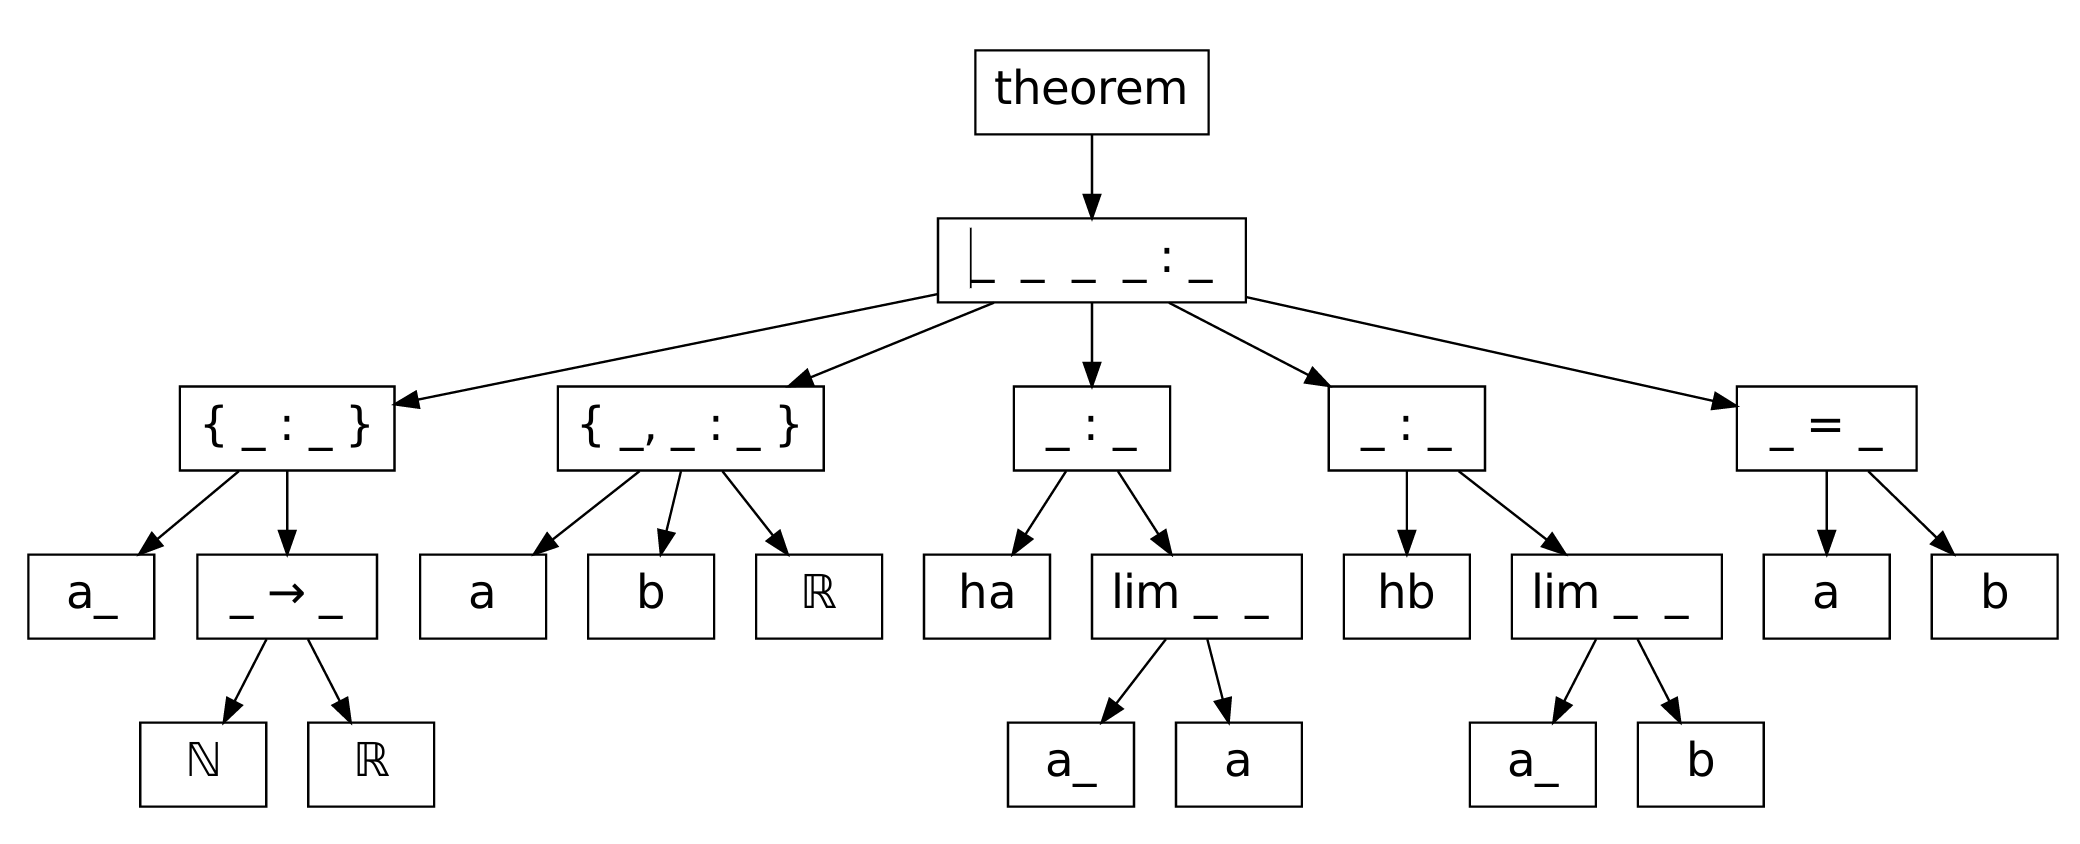
\includegraphics[width=0.5\textwidth]{figures/operator tree.png}
            \label{fig:OperatorTree2}
            \caption{完整复原的算子树}
        \end{figure}

        \textbf{大语言模型 (\underline{L}arge \underline{L}anguage \underline{M}odel (LLM))} 技术成熟后, 自动形式化技术兴起. 北京大学团队的 Herald 模型\footnote{https://arxiv.org/pdf/2410.10878}与上海交大团队的 ATLAS 模型\footnote{https://arxiv.org/pdf/2502.05567}是代表性的自动形式化模型. 

    \subsection{证明状态变换}
        
        接下来我们将介绍一阶逻辑算子的证明状态变换, 以及在 Lean 中如何使用这些变换来进行形式化证明. 介绍一阶形式逻辑时, 用类似 Gentzen 相继式演算的书写方式表意, 但一些左右规则做了适当简化. 

        \begin{syn}
            {变量声明}
            在 Lean 中, 使用 \lean{variable} 关键字可以全局声明变量, 这样就无需在定理声明时反复声明相同的变量: 
            \begin{lstlisting}[style=lean]
    variable (p q : Prop)
    theorem #tm{pq} : p → q := by sorry
            \end{lstlisting}

            但需要注意, 这样声明的定理仍是依值函数, 在使用时仍需提供参数: 
            \begin{lstlisting}[style=lean]
    #check pq       --  ∀ (p q : Prop), p → q
    theorem #tm{sth} (hp : p) : q := pq hp  -- error
            \end{lstlisting}

            若隐式声明变量, 则不会有这个问题. 我们下文中默认 $p,q,r$ 指代命题. 
            \begin{lstlisting}[style=lean]
    variable {p q r : Prop}
            \end{lstlisting}
        \end{syn}

    我们用蓝色 ``$\Goal$'' 表示 Lean 策略证明中的 ``证明状态'', ``$\longrightarrow$'' 表示证明状态变换, 含义为 ``要证明 \dots 只需证明 \dots''. 注意证明状态变化的方向和实际推理中证明合成的方向是相反的. 
        
        \begin{axm}
            {切割规则}
            {Cut}
            若语境下命题 $p$ 有证明, 借助命题 $p$ 的证明能构造命题 $q$ 的证明, 则语境下能直接构造命题 $q$ 的证明: 
            \[\frac{\Gamma\vdash(h_p : p)\qquad\Gamma,(h_p : p)\vdash(h_q : q)}{\Gamma\vdash(h_q : q)}\]
        \end{axm}
    
        \begin{tactic}
            {引理引入}
            使用 \lean{have} 策略可以构造一个新的引理以帮助证明目标: 
            \begin{lstlisting}[style=lean]
    theorem th_name {p : Prop} : q := by
      have hp : p := by sorry
      #check hp         --  p
      sorry
            \end{lstlisting}

            \lean{have} 策略内是一个独立的证明状态, 其证明目标为 \texttt{p}, 证明完成后会将 \texttt{hp} 添加到当前语境中. 
        \end{tactic}
        
        \begin{axm}
            {合取右规则}
            {Right Rule of Conjunction}
            若命题 $p$ 和 $q$ 均有证明, 则可构造一个命题 $p\land q$ 的证明: 
            \[\frac{\Gamma\vdash(h_p : p)\qquad\Gamma\vdash(h_q : q)}{\Gamma\vdash(h : p\land q)}(\land R)\]
        \end{axm}

        \begin{tactic}
            {合取证明目标的处理}
            合取右规则对应以下证明状态的变化: 
            \[\Gamma\Goal(p\land q)\quad\longrightarrow\quad
            \begin{cases}
                (\Gamma\Goal p)\\
                (\Gamma\Goal q)
            \end{cases}\]
            
            可使用 \lean{constructor} 策略拆分合取证明目标: 
            \begin{lstlisting}[style=lean]
    theorem #tm{Conj_constructor} (hp : p) (hq : q) : p ∧ q := by
      constructor       -- Goal_1 : p, Goal_2 : q
      · exact hp
      · exact hq
            \end{lstlisting}
            
            也可使用 \lean{refine} 策略与语法缺口来构造合取证明目标: 
            \begin{lstlisting}[style=lean]
    theorem #tm{Conj_refine} (hp : p) (hq : q) : p ∧ q := by
      refine ⟨?_, ?_⟩    -- Goal_1 : p, Goal_2 : q
      · exact hp
      · exact hq
            \end{lstlisting}
        \end{tactic}

        \begin{axm}
            {合取左规则}
            {Left Rules of Conjunction}
            若可用一个命题 $p$ 的证明构造结论的证明, 则可用 $p\land q$ 的证明构造结论的证明: 
            \[\frac{\Gamma\vdash(h_p : p)}{\Gamma, (h : p\land q)\vdash G}(\land L_1)\]

            若可用一个命题 $q$ 的证明构造结论的证明, 则可用 $p\land q$ 的证明构造结论的证明:
            \[\frac{\Gamma\vdash(h_q : q)}{\Gamma, (h : p\land q)\vdash G}(\land L_2)\]
        \end{axm}

        \begin{tactic}
            {合取假设的处理}
            合取左规则对应以下证明状态变化: 
            \[\Gamma, (h : p\land q)\Goal r\quad\longrightarrow\quad\Gamma, (h : p\land q), (h_p : p), (h_q : q)\Goal r\]

            可使用 \lean{have} 策略解析合取假设: 
            \begin{lstlisting}[style=lean]
    theorem #tm{Conj_have1} (h : p ∧ q) : p := by
      have ⟨hp, hq⟩ := h
      exact hp

    theorem #tm{Conj_have2} (h : p ∧ q) : p := by
      have hp : p := h.left
      have hq : q := h.right
      exact hp

    theorem #tm{Conj_have3} (h : p ∧ q) : p := by
      have hp : p := h.1
      have hq : q := h.2
      exact hp
            \end{lstlisting}

            \lean{have} 策略会保留原合取命题的证明 $h : p\land q$, 但下两种方式会将之丢弃, 即对应以下证明状态变化: 
            \[\Gamma, (h : p\land q)\Goal r\quad\longrightarrow\quad\Gamma, (h_p : p), (h_q : q)\Goal r\]
            
            也可使用 \lean{obtain} 和 \lean{rcases} 策略解析合取假设: 
            \begin{lstlisting}[style=lean]
    theorem #tm{Conj_rcases} (h : p ∧ q) : p := by
      rcases h with ⟨hp, hq⟩
      exact hp

    theorem #tm{Conj_obtain} (h : p ∧ q) : p := by
      obtain ⟨hp, hq⟩ := h
      exact hp
            \end{lstlisting}
        \end{tactic}
        

        \begin{axm}
            {蕴含右规则}
            {Right Rule of Implication}
            若在有命题 $p$ 的证明时可构造一个命题$q$ 的证明, 则可构造一个命题 $p\to q$ 的证明: 
            \[\frac{\Gamma, (h_p : p)\vdash(h_q : q)}{\Gamma\vdash(h : p\to q)}(\to R)\]
        \end{axm}

        \begin{tactic}
            {蕴含证明目标的处理}
            蕴含右规则对应证明状态变化: 
            \[\Gamma\Goal(p\to q)\quad\longrightarrow\quad\Gamma, (h_p : p)\Goal q\]
            
            可使用 \lean{intro} 策略来提取蕴含命题的假设: 
            \begin{lstlisting}[style=lean]
    theorem #tm{Imp_intro} (hq : q) : p → q := by
      intro hp
      exact hq
            \end{lstlisting}
            
            也可使用 \lean{refine} 策略与语法缺口来构造合取证明目标: \footnote{$\lambda$-抽象的演算语法将在第三章具体讲解. }
            \begin{lstlisting}[style=lean]
    theorem #tm{Imp_refine_left} (hq : q) : p → q := by
      refine fun hp => ?_
      exact hq
            \end{lstlisting}
        \end{tactic}

        \begin{axm}
            {蕴含左规则}
            {Left Rule of Implication}
            若命题 $p$ 有证明, 则可用 $p\to q$ 的证明构造一个命题 $q$ 的证明: 
            \[\frac{\Gamma\vdash(h_p : p)}{\Gamma,(h : p\to q)\vdash q}(\to L)\]
        \end{axm}

        \begin{tactic}
            {蕴含假设的处理}
            蕴含左规则以下证明状态变化: 
            \[\Gamma, (h : p\to G)\Goal G\quad\longrightarrow\quad\Gamma, (h : p\to G)\Goal p\]
            
            可使用 \lean{apply} 策略来应用蕴含假设: 
            \begin{lstlisting}[style=lean]
    theorem #tm{Imp_apply} (hp : p) (h : p → q) : q := by
      apply h
      exact hp
            \end{lstlisting}

            也可使用 \lean{refine} 策略与语法缺口来更改证明目标: 
            \begin{lstlisting}[style=lean]
    theorem #tm{Imp_refine_right} (hp : p) (h : p → q) : q := by
      refine h ?_
      exact hp
            \end{lstlisting}
        \end{tactic}

        \begin{axm}
            {析取右规则}
            {Right Rule of Disjunction}
            若命题 $p$ 有证明, 则可构造一个命题 $p\lor q$ 的证明: 
            \[\frac{\Gamma\vdash(h_p : p)}{\Gamma\vdash(h : p\lor q)}(\lor R_1)\]

            若命题 $q$ 有证明, 则可构造一个命题 $p\lor q$ 的证明: 
            \[\frac{\Gamma\vdash(h_q : q)}{\Gamma\vdash(h : p\lor q)}(\lor R_2)\]
        \end{axm}

        \begin{tactic}
            {析取证明目标的处理}
            析取右规则对应以下证明状态变化: 
            \[\Gamma\Goal(p\lor q)\quad\longrightarrow\quad(\Gamma\Goal p);\qquad\Gamma\Goal(p\lor q)\quad\longrightarrow\quad(\Gamma\Goal q)\]
            使用 \lean{left} / \lean{right} 策略选择析取的左 / 右分支: 
            \begin{lstlisting}[style=lean]
    theorem #tm{Disj_left} (hp : p) : p ∨ q := by
      left          -- Goal : p
      exact hp

    theorem #tm{Disj_right} (hq : q) : p ∨ q := by
      right         -- Goal : q
      exact hq
            \end{lstlisting}
        \end{tactic}

        \begin{axm}
            {析取左规则}
            {Left Rule of Disjunction}
            若用 $p$ 和 $q$ 可分别合成出 $r$ 的证明, 则可用命题 $p\lor q$ 的证明构造一个命题 $r$ 的证明: 
            \[\frac{\Gamma, (h_p : p)\vdash(h_r : r)\qquad\Gamma, (h_q : q)\vdash(h_r : r)}{\Gamma, (h : p\lor q)\vdash(h_r : r)}(\lor L)\]


        \end{axm}

        \begin{tactic}
            {析取假设的处理}
            析取左规则对应以下证明状态变化: 
            \[\Gamma, (h : p\lor q)\Goal G\quad\longrightarrow\quad
            \begin{cases}
                (\Gamma, (h_p : p)\Goal G)\\
                (\Gamma, (h_q : q)\Goal G)
            \end{cases}\]
            
            可使用 \lean{obtain} 策略或 \lean{rcases} 策略对析取假设分类讨论: 
            \begin{lstlisting}[style=lean]
    theorem #tm{Disj_obtain} (h : p ∨ q)(pr : p → r)(qr : q → r): r := by
      obtain hp | hq := h
      · exact pr hp
      · exact qr hq

    theorem #tm{Disj_rcases} (h : p ∨ q)(pr : p → r)(qr : q → r): r := by
      rcases h with hp | hq
      · exact pr hp
      · exact qr hq
            \end{lstlisting}
        \end{tactic}

        \begin{axm}
            {全称量词右规则}
            {Right Rule of Universal Quantifier}
            若 $a$ 是 $\alpha$ 的元素且不在语境中, $p$ 是 $\alpha$ 上的一元谓词, 命题 $p(a)$ 有一个证明, 则可构造一个命题 $\forall x : \alpha, p(x)$ 的证明: 
            \[\frac{\Gamma, (a : \alpha)\vdash(h_p : p(a))}{\Gamma\vdash\forall x : \alpha, p(x)}(\forall R)\]
        \end{axm}

        \begin{tactic}
            {全称量词证明目标的处理}
            全称量词右规则对应以下证明状态变化: 
            \[\Gamma\Goal(\forall x : \alpha, p(x))\quad\longrightarrow\quad\Gamma, (a : \alpha)\Goal p(a)\]

            可使用 \lean{intro} 策略将全称量词目标实例化: 
            \begin{lstlisting}[style=lean]
    theorem Forall_intro : ∀ x, P x := by
      intro x       --  Goal: P x
      #check x      --  x : α
      sorry
            \end{lstlisting}
            
            也可使用 \lean{refine} 策略创造语法缺口: 
            \begin{lstlisting}[style=lean]
    theorem Forall_refine : ∀ x, P x := by
      refine fun x => ?_  -- Goal: P x
      #check x            -- x : α
      sorry
            \end{lstlisting}
        \end{tactic}

        \begin{axm}
            {全称量词左规则}
            {Left Rule of Universal Quantifier}
            若 $p$ 是 $\alpha$ 上的一元谓词, $a$ 是类型为 $\alpha$ 的元素, 命题 $p(a)$ 有证明, $a$ 是 $\alpha$ 的元素, 则可构造一个命题 $p(a)$ 的证明: 
            \[\frac{\Gamma,(a : \alpha), (h_p : p(a))\vdash q}{\Gamma, (h : \forall x : \alpha, p(x)), (a : \alpha)\vdash q}(\forall L)\]
        \end{axm}

        \begin{tactic}
            {全称量词假设的处理}
            全称量词左规则对应以下证明状态变化: 
            \[\Gamma, (a : \alpha), (h : \forall x : \alpha, P(x))\Goal p\quad\longrightarrow\quad\Gamma, (a : \alpha), (h : \forall x : \alpha, P(x)), (h_p : P(a))\Goal p\]

            可以对全称量词假设代入具体变量: 
            \begin{lstlisting}[style=lean]
    theorem Forall_sub (h : ∀ x, P x) (a : α) : p := by
      #check h a          -- P a
      sorry     
            \end{lstlisting}

            特别地, 当证明目标与全称量词代入的结果相同时, 可以直接使用 \lean{apply} 策略. 原则上需要提供一个 $\alpha$ 类型的实例, 但实际上 Lean 会自动推断并直接完成证明: 
            \[\Gamma, (a : \alpha), (h : \forall x : \alpha, P(x))\Goal P(a)\quad\longrightarrow\quad\Gamma, (h : \forall x : \alpha, P(x))\Goal\alpha\quad\longrightarrow\quad\lean{No Goals}\]
            \begin{lstlisting}[style=lean]
    theorem Forall_apply (h : ∀ x, P x) (x : α) : P x := by
      apply h
            \end{lstlisting}
        \end{tactic}

        \begin{axm}
            {存在量词右规则}
            {Right Rule of Existential Quantifier}
            若 $a$ 是 $\alpha$ 的元素, $p$ 是 $\alpha$ 上的一元谓词, 命题 $p(a)$ 有一个证明, 则可构造一个命题 $\exists x : \alpha, p(x)$ 的证明: 
            \[\frac{\Gamma(a : \alpha)\vdash(h_p : p(a))}{\Gamma(a : \alpha)\vdash(\exists x : \alpha, p(x))}(\exists R)\]
        \end{axm}

        \begin{tactic}
            {存在量词证明目标的处理}
            以下证明状态变化: 
            \[\Gamma, (a : \alpha)\Goal(\exists x : \alpha, p(x))\quad\longrightarrow\quad\Gamma, (a : \alpha)\Goal p(a)\]
            \[\Gamma\Goal(\exists x : \alpha, p(x))\quad\longrightarrow\quad(\Gamma\Goal(a : \alpha)), (\Gamma\Goal p(a))\]
            
            可使用 \lean{use} 策略提供实例: 
            \begin{lstlisting}[style=lean]
    theorem Exists_use (a : α) : ∃ x, P x := by
      use a               -- Goal: P a
      sorry
            \end{lstlisting}
            
            也可使用 \lean{refine} 策略创造语法缺口, 依值对的依赖关系会被保留: 
            \begin{lstlisting}[style=lean]
    theorem Exists_refine (a : α) : ∃ x, P x := by
      refine ⟨?_, ?_⟩
      · exact a            -- Remaining Goal: P a
      · sorry
            \end{lstlisting}

            使用 \lean{constructor} 搭配 \lean{case} 策略也可以实现同样效果: \footnote{我没有搞明白为什么依值对中的变量会自动变成第二个目标. }
            \begin{lstlisting}[style=lean]
    theorem Exists_constructor (a : α) (h : P a) : ∃ x, P x := by
      constructor
      case w => exact a
      · sorry
            \end{lstlisting}
        \end{tactic}

        \begin{axm}
            {存在量词左规则}
            {Left Rule of Existential Quantifier}
            若命题 $\exists x : \alpha, p(x)$ 有证明, 则可构造一个类型为 $\alpha$ 的元素 $a$ 和一个命题 $p(a)$ 的证明: 
            \[\frac{\Gamma, (h : \exists x : \alpha, P(x))\vdash(h_p:p)}{\Gamma, (a : \alpha),(h : P(a))\vdash(h_p:p)}(\exists L)\]
        \end{axm}

        \begin{tactic}
            {存在量词假设的处理}
            存在量词右规则对应以下证明状态变化: 
            \[\Gamma, (h : \exists x : \alpha, p)\Goal G\quad\longrightarrow\quad\Gamma, (a : \alpha), (h_p : p(a)), (h : \exists x : \alpha, p)\Goal G\]

            使用 \lean{have}, \lean{obtain} 或 \lean{rcases} 策略解析存在量词假设: 
            \begin{lstlisting}[style=lean]
    theorem Exists_have (h : ∃ x, P x) : p := by
      have ⟨a, ha⟩ := h
      sorry

    theorem Exists_obtain (h : ∃ x, P x) : p := by
      obtain ⟨a, ha⟩ := h
      sorry

    theorem Exists_rcases (h : ∃ x, P x) : p := by
      rcases h with ⟨a, ha⟩
      sorry
            \end{lstlisting}

            以上三种方式与合取假设的处理大同小异. 除 \lean{have} 策略外, 其他策略会导致原存在量词假设丢失. 
        \end{tactic}

        \begin{axm}
            {矛盾律与排中律}
            {Contradiction and Law of Excluded Middle}
            命题 $\neg p$ 定义为 $p$ 蕴含矛盾: 
            \[\neg p := p\to\texttt{False}\]

            若 $p$ 和 $\neg p$ 同时有证明, 则可构造一个矛盾的证明, 进而可构造任何命题的证明: 
            \[\frac{}{\Gamma, (h_1 : p), (h_2 : \neg p)\vdash\texttt{False}}\]

            $p$ 和 $\neg p$ 中总有一个有证明, 即: 
            \[\frac{\Gamma,(h_1:p)\vdash (h_q:q)\qquad\Gamma,(h_2:\neg p)\vdash (h_q:q)}{\Gamma\vdash(h_q:q)}\]
        \end{axm}

        \begin{tactic}
            {否定算子的处理}
            使用 \lean{intro} 策略处理否定算子的定义: (不依赖排中律)
            \begin{lstlisting}[style=lean]
    theorem Not_intro : ¬p := by
      intro h
      sorry
            \end{lstlisting}

            当假设中有矛盾时, 使用 \lean{contradiction} 策略结束证明: 
            \begin{lstlisting}[style=lean]
    theorem Not_contradiction (h1 : p) (h2 : ¬p) : q := by
      contradiction

    theorem False_contradiction (h : False) : q := by
      contradiction
            \end{lstlisting}

            排中律允许使用反证法证明命题 (\lean{contrapose!} 策略和 \lean{by\_contra} 策略): 
            \begin{lstlisting}[style=lean]
    theorem Not_contrapose (h1 : p) (h2 : ¬p) : q := by
      contrapose! h2
      exact h1

    theorem Not_by_contra : p := by
      by_contra h
      sorry
            \end{lstlisting}

            排中律允许使用 \lean{by\_cases} 策略进行分类讨论, 对应的证明状态变化: 
            \[\Gamma\Goal q\quad\longrightarrow\quad
            \begin{cases}
                (\Gamma(h : p)\Goal q)\\
                (\Gamma(h : \neg p)\Goal q)
            \end{cases}\]
            \begin{lstlisting}[style=lean]
    theorem By_cases {p : Prop} : q := by
      by_cases h : p
      · sorry
      · sorry
            \end{lstlisting}
        \end{tactic}
        
            
\end{document}